\graphicspath{ {./images/} }
\chapter{設計}
\label{c:design}

{\color{red}
無狀態區塊鏈為了縮減硬碟佔用空間,必須在交易附上證明,導致所需網路流量增大;
為了省去硬碟隨機存取所耗用的時間,必須花費 CPU 計算能力來驗證證明。

無狀態區塊鏈相較於一般區塊鏈做出了一些取捨(trade-off),
而淺狀態區塊鏈的目的是讓這種取捨不再是全有或全無(全部都附上證明或全部不附上證明),
使得狀態儲存的程度變得可調節。
}

\section{淺狀態區塊鏈}

{\color{red}
無狀態區塊鏈中的一個區塊,如果多份交易的付款人、收款人都相同,
交易的證明也會是完全相同的,這樣重複的資訊顯然可以省略。

擴展這個想法,如果我們快取最近出現過的交易中的賬戶資訊,
則下一次收到同樣賬戶的交易時,也不需要去驗證證明。

再更進一步,讓整個網路上的節點都遵循同一套規則來記錄快取,
使得所有節點對於什麼時候要附證明、什麼時候不用附證明有共識,
那在區塊廣播的時刻,節點就能夠剝離掉不必要的證明,進而省下區塊的流量。
}

TODO: 補以太坊交易的快取分析圖

TODO: 分析 trade-off 記憶體速度很快

如果節點在驗證同一個區塊時,使用的快取不一致,
將會導致某些節點承認該區塊,某些節點不承認,從而導致分叉。

譬如,如果節點快取住它高度最高的 k 個區塊中的交易資訊,
當網路延遲,不同節點中的鏈分叉情形不同時,快取就會不一致,見下圖:

\begin{figure}[h]
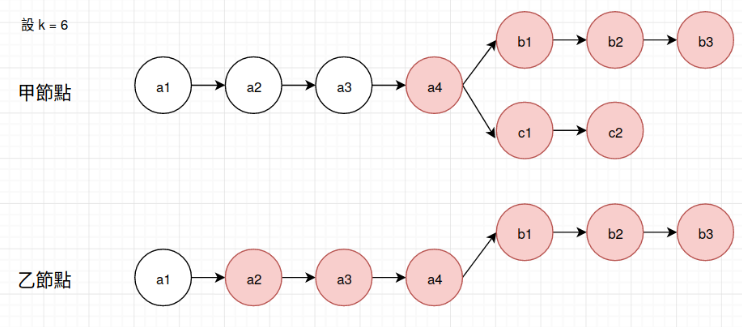
\includegraphics[width=\textwidth]{wrong-cache}
\caption{不一致的快取}
\end{figure}

粉紅色表示在快取,白色區塊則表示不在快取。
此時若有一個不附證明的交易,付款方在 a2 區塊出現過,則乙節點會接收交易,甲節點則不會接收。

\section{快取設計}

{\color{red}
一個簡單的設計準則可以避免前述的錯誤:每一個區塊都有自己的快取,
快取的內容僅僅由該區塊所在的鏈的資料所決定。如此,我們把樹狀結構縮減為一個串列(list),
而不同節點上同個區塊所在的串列必定是相同的,只要每個節點都用同樣的確定性算法從這個串列計算出快取,
就能夠保證每個節點驗證同一個區塊時的快取一致。
}

\subsection{分叉處理}

觀察以下這條鏈:

\begin{figure}[h!]
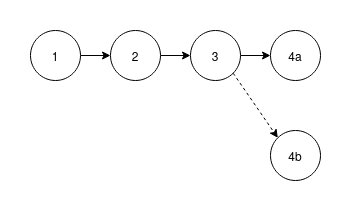
\includegraphics[width=10cm]{快取分叉}
\caption{區塊鏈分叉}
\end{figure}

此時,區塊 4b 嘗試接上區塊 3 ,因此它必須基於區塊 3 的快取來進行驗證。
也就是說,如果我們在接上區塊 4a 時,將區塊 3 的快取直接修改而稱為區塊 4a 的快取,
那當我們要街區塊 4b 時,就無從知悉區塊 3 的快取了,使用某些快取策略時,
我們可以透過回退(roll back)來取回區塊 3 的快取,但當使用某些快取策略時,遺失的快取無法輕易找回。

即使使用可以回退的快取策略,當分支切換越頻繁,回退的次數也會越頻繁,
而回退的效能可能就會成為瓶頸。

例如在圖 3.3 中,如果同時維持 a, b 兩條分支,則每次接收到非當前分叉的區塊時,都要進行回退,
並且隨著分叉的差異越大,回退的長度也越長,若從 7a 要走到 7b ,就必須先退回 3 ,再走回 7b ,
若之前曾經從 6a 走到過 6b ,則過程中的大部分運算都是相同的,這顯然是一種浪費。

\begin{figure}[h!]
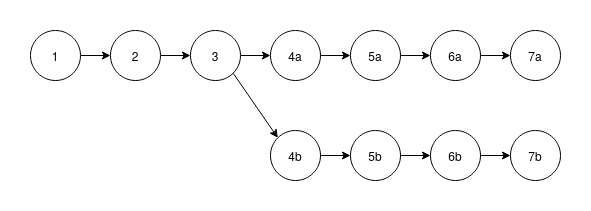
\includegraphics[width=\textwidth]{快取長分叉}
\caption{分叉頻繁切換}
\end{figure}

{\color{red}
\subsection{持久化快取}

我們採用另外一種思路:在每個區塊上都保留它自己的快取,當新區塊要接上鏈的時候,
就可以直接取用它前一個區塊的快取,無需重新計算。
換句話說,我們採用全持久化資料結構(fully persistent data structure)~\cite{driscoll1986making}來儲存快取,
每接受一個區塊,就生成一個快取的版本。

在這個方案中,我們必須定時刪除太舊(例如,距離最長鏈超過 20 個區塊)區塊的快取,
以將整條鏈的快取大小限制在一定範圍,否則任由快取無限增長,將導致記憶體用罄,
以致於必須使用到硬碟,快取就變得沒有意義了。

這個方案帶來了一個立即問題,如果我們每次都複製前一個區塊的快取,
那快取的所佔用的空間將會正比於未刪除的快取的數量。
然而,相鄰區塊中的快取有很高的相似性,若能選用適當的資料結構來讓相鄰區塊共享快取,
將能夠有效提高空間使用率。
}

\section{快取策略}

不同的快取策略在應對不同工作量(workload)時的命中率(hit rate)各不相同,
以下討論實作簡單的「最近 k 塊」策略、FIFO 策略,以及實作較為複雜,但經驗上命中率較高的 LRU 策略。

\subsection{最近 k 塊}

在「最近 k 塊」策略中,一個區塊的快取即為由該區塊開始,由高往低取 k 個區塊,
這 k 個區塊中出現過的交易中的資訊。

以下為 k = 6 的示意圖

\begin{figure}[h]
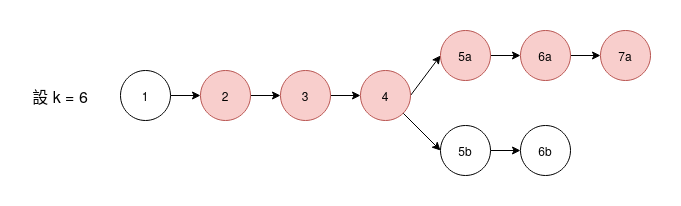
\includegraphics[width=\textwidth]{最近k塊}
\caption{區塊 7a 為粉紅色區塊中的所有交易資訊}
\end{figure}

可以用一個鍵值對(key value pairs)(其底層可為雜湊表(hash table)、平衡搜尋樹(balenced search tree)、跳錶(skip list)......等等)來表示快取,
若考慮每次重算的情境,例如在圖 3.4 中,要在 7a 後方額外加入一個 8a 區塊,
則我們加入 8a 區塊中的交易資訊,並丟掉只在 6a 中出現但沒有在其餘區塊中出現的交易資訊。

「最近 k 塊」的快取可以回退,跟前進時的算法一樣,只是換了個方向。

當考慮全持久化時,我們可以選用可持久化的鍵值對資料結構,
例如雜湊\cite{bagwell2001ideal}\cite{puente2017persistence}、搜尋樹都有相對應高效成熟的持久化實作,
若一個快取有 n 個鍵,則持久化雜湊/搜尋樹插入/刪除一筆鍵值時,
時間、空間複雜度皆為 $O(log(n))$。

\subsection{FIFO}

\subsection{LRU}

{\color{red}
LRU 是 least recently used 的縮寫,這種策略中,快取大小是固定的,
若快取已滿,在插入新資料之前必須先丟棄一筆資料,
LRU 會去挑選快取中所有資料中最久沒被用到的那一筆來丟棄。

LRU 之所以比 FIFO 的命中率更高,是因為以太坊的歷史數據顯示,
(1) 一個賬戶花錢之後,很可能又接著花錢。 (2) 一個賬戶收到錢之後,
很可能會馬上將錢花掉。LRU 由於會更新資料的使用時間,得以一直快取住頻繁出現的資料,
FIFO 則只看資料進入快取的時間,只要快取失效會發生,
快取需要被抽換,那即使某些資料頻繁出現,遲早還是會被丟掉。

進一步抽象來看, LRU 是一種支援兩個介面的資料結構,

\begin{itemize}
  \item get(key)
  \item put(key, value)
\end{itemize}

get(key) 時,若 LRU 存在該鍵,則返回對應值,並且將 key 的使用時間調整到最新。

put(key, value) 時,若 LRU 空間未滿,直接插入一筆鍵值對,
這筆新鍵值對的的使用時間為最新;若 LRU 空間已滿,
就要找出當前快取中使用時間最舊的丟掉,再插入新鍵值對,此新鍵值對的使用時間亦為最新。

對應到淺狀態區塊鏈的情境中,每當一個區塊要接上,我們要計算新區塊快取時,
會把一系列帳號資訊的讀取跟修改操作轉變成 get 跟 put ,鍵是帳號地址,值是帳號狀態,
然後在 LRU 底層的資料結構上進行相應操作。
}

當在淺狀態區塊鏈中使用 LRU 策略時,是無法回退的,其原因為 TODO

\section{持久化 LRU 算法}
在討論持久化 LRU 算法之前,我們先觀察如何在軟體上高效實作 LRU 快取,
調查 github 上多個高使用量的 LRU 函式庫,內部資料結構都是雜湊表與雙向鏈表(doubly linked list)的組合:

\begin{figure}[h]
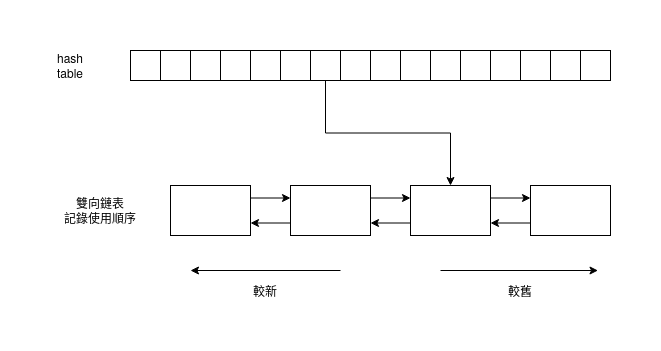
\includegraphics[width=\textwidth]{LRU}
\caption{LRU 資料結構}
\end{figure}

TODO: 補圖

執行 get 時,透過雜湊得到指向值的指針,獲取資料,並且將指針指向的鏈表節點移動至鏈表頭部(最左側)。
執行 put 時,若快取命中,更新節點的值,並將節點移動至鏈表頭部,
若快取未滿,從頭部加入快取值,並將其指針放入雜湊表,
若快取已滿,拔出雙向鏈表的尾部(最右側)節點,並且在雜湊表中移除該舊鍵,
然後在頭部加入快取值,放指針到雜湊表。

觀察到 LRU 需要記錄的資訊有二:

\begin{enumerate}
  \item 由鍵找到值(鍵值對)
  \item 各個鍵的順序資訊
\end{enumerate}

在前述的雜湊表 + 雙向鏈表的實現方案中,雜湊表負責 (1) ,雙向鏈表則負責 (2),
注意到,雙向鏈表極為自然的記錄了順序關係,它甚至不需要記錄確切的擷取時間。

一個簡單的想法是,我們直接把雜湊跟雙向鏈表的持久化替代品組合起來,
就得到了一個持久化 LRU ,然而,雖然持久化雜湊有很成熟的替代品,
持久化雙向鏈表卻沒有。

因此,我們需要用其他可高效持久化的資料結構來取代雙向鏈表,進一步抽象雙向鍵表做的事情有:

\begin{itemize}
  \item 更新一個節點的使用時間到最新
  \item 刪除使用時間最舊的節點
  \item 插入新節點,新節點的使用時間為最新
\end{itemize}

以下,先討論了如何用紅黑樹\cite{guibas1978dichromatic}(平衡搜尋樹)來完成上述任務,
再介紹我們設計的順序樹資料結構,相比紅黑樹,它更加高效。

\subsection{雜湊 + 紅黑樹}

我們嘗試使用紅黑樹來記錄順序資訊。首先,為每一筆賬戶資訊設置一個獨一無二的時間序,
這個時間序可以很容易得到,例如說設置成 $block\_height * max\_tx\_in\_one\_block + tx\_number$。

然後,以時間序做為鍵,賬戶資訊為值,建造一棵紅黑樹。雜湊表則用賬戶地址為鍵,對應的時間序為值。

get 時,先在雜湊表中由賬戶地址得到時間序,再到紅黑樹中由時間序得到賬戶資訊。
例如,在圖 3.6 中,我們會先從雜湊表得到賬戶的時間序為 243 ,再到紅黑樹中查找 243 。

\begin{figure}[h!]
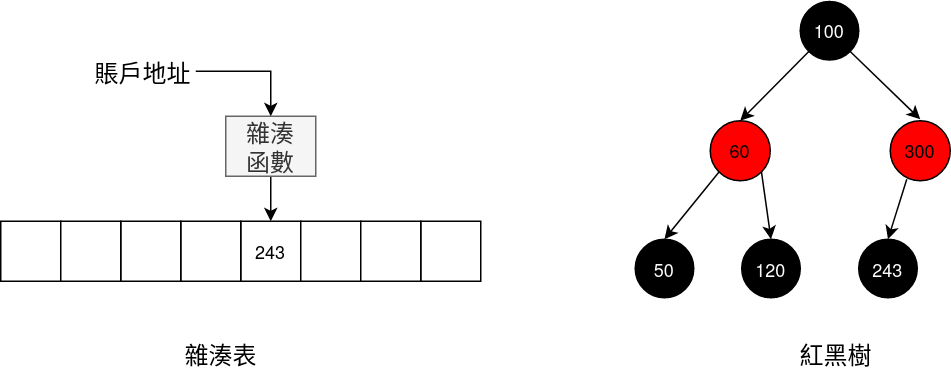
\includegraphics[width=\textwidth]{雜湊紅黑樹}
\caption{雜湊 + 紅黑樹}
\end{figure}

查找後,需更新使用時間。具體操作爲修改雜湊表中地址對應的時間序,
並移除紅黑樹中的原節點,加入新時間序做為鍵。

put 類似於 get ,但需要修改賬戶資訊。

圖 3.6 表示不可變紅黑樹的共享結構。該圖中,快取的大小設爲 8 。
狀態 1 時,只有 7 筆資料,狀態 2 對狀態 1 插入 14 ,資料變成 8 筆,
狀態 3 再對狀態 2 插入 15 ,由於快取已滿,必須先刪除時間序最小的資料,
也就是最左下角的紅色 7 。

\begin{figure}[h!]
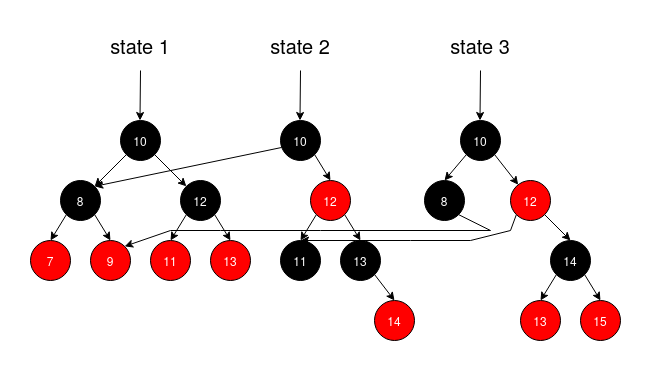
\includegraphics[width=\textwidth]{不可變紅黑樹}
\caption{不可變紅黑樹}
\end{figure}

\subsubsection{紅黑樹 bulk 優化}

\subsection{雜湊 + 順序樹}

雙向鏈接串列以節點之間的指向關係記錄順序關係,紅黑樹卻必須額外記錄時間序,
此外,原本透過雜湊就能一次查找到賬戶資訊,紅黑樹方案卻得\emph{地址 -> 時間序 -> 賬戶資訊}兩段式地查找。

雙向鏈表無法以路徑複製來變換爲不可變資料結構的原因在於,
兩個相鄰節點總是互指,一旦以路徑複製的方式修改節點,就得複製整個鏈表。
於是我們思考,不要用互指的方式來連接節點,就可以順利路徑複製。

想像在這些節點的背後編織一張網,然後將它們粘在一起(圖 3.8)。

\begin{figure}[h!]
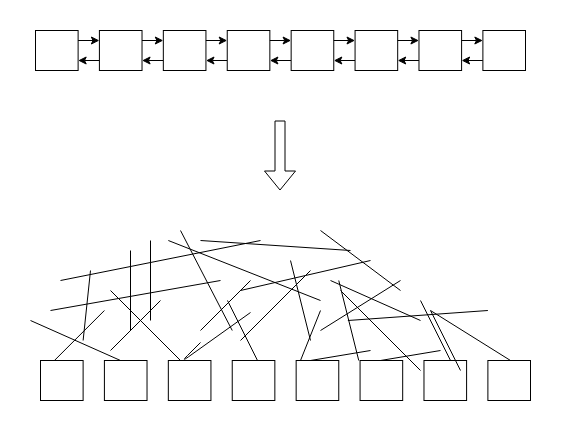
\includegraphics[width=\textwidth]{節點網}
\caption{}
\end{figure}

這個網狀結構最簡單形式就是一棵滿二元樹(full binary tree)(圖 3.8)。

\begin{figure}[h!]
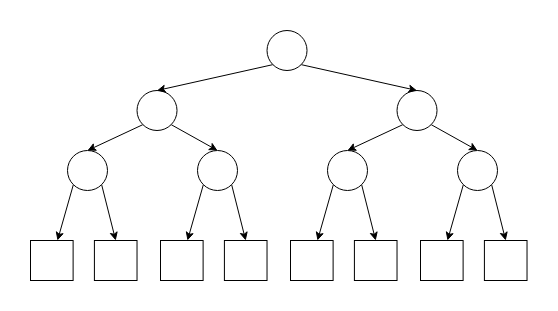
\includegraphics[width=\textwidth]{滿二元樹}
\caption{滿二元樹連接節點}
\end{figure}

我們將利用滿二元樹來儲存順序資訊的資料結構稱爲順序樹,
以下開始一一介紹順序樹的各種操作。

若快取的容量爲 $n$ ,順序樹的高度將會設置爲 $1 + \lceil \log_2 n \rceil$,
也就是說,葉子的數量至少是快取容量的兩倍。圖 3.10 就是一棵容量爲 4 的順序樹,它有 8 個葉子節點。

\begin{figure}[h!]
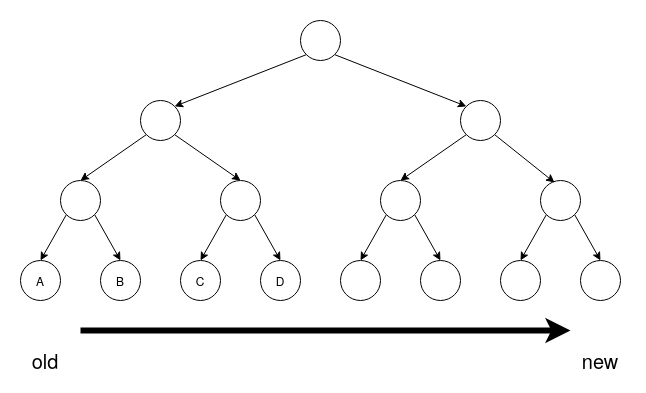
\includegraphics[width=\textwidth]{順序樹}
\caption{容量爲 4 的順序樹}
\end{figure}